% AER E 361 Mission Report Template
% Spring 2023
% Template created by Yiqi Liang and Professor Matthew Nelson

% Document Configuration DO NOT CHANGE
\documentclass[12 pt]{article}
% --------------------LaTeX Packages---------------------------------
% The following are packages that are used in this report.
% DO NOT CHANGE ANY OF THE FOLLOWING OR YOUR REPORT WILL NOT COMPILE
% -------------------------------------------------------------------

\usepackage{hyperref}
\usepackage{parskip}
\usepackage{titlesec}
\usepackage{titling}
\usepackage{graphicx}
\usepackage{graphviz}
\usepackage[T1]{fontenc}
\usepackage{titlesec, blindtext, color} %for LessIsMore style
\usepackage{tcolorbox} %for references box
\usepackage[hmargin=1in,vmargin=1in]{geometry} % use 1 inch margins
\usepackage{float}
\usepackage{tikz}
\usepackage{svg} % Allows for SVG Vector graphics
\usepackage{textcomp, gensymb} %for degree symbol
\hypersetup{
	colorlinks=true,
	linkcolor=blue,
	urlcolor=cyan,
}
\usepackage{biblatex}
\addbibresource{lab-report-bib.bib}
\usepackage{amsmath}
\usepackage{listings}
\usepackage{multicol}
\usepackage{array}

\usepackage{hologo} %KYR: for \BibTeX
%\usepackage{algpseudocode}
%\usepackage{algorithm}
% This configures items for code listings in the document
\usepackage{xcolor}

\usepackage{fancyhdr} % Headers/Footers
\usepackage{siunitx} % SI units
\usepackage{csquotes} % Display Quote
\usepackage{microtype} % Better line breaks
\usepackage{mathtools} % Gives more math symbols

\definecolor{commentsColor}{rgb}{0.497495, 0.497587, 0.497464}
\definecolor{keywordsColor}{rgb}{0.000000, 0.000000, 0.635294}
\definecolor{stringColor}{rgb}{0.558215, 0.000000, 0.135316}
\definecolor{mygreen}{rgb}{0,0.6,0}
\definecolor{mygray}{rgb}{0.5,0.5,0.5}
\definecolor{mymauve}{rgb}{0.58,0,0.82}

\lstdefinestyle{customc}{
  belowcaptionskip=1\baselineskip,
  breaklines=true,
  frame=L,
  xleftmargin=\parindent,
  language=C,
  showstringspaces=false,
  basicstyle=\footnotesize\ttfamily,
  keywordstyle=\bfseries\color{green!40!black},
  commentstyle=\itshape\color{purple!40!black},
  identifierstyle=\color{blue},
  stringstyle=\color{orange},
 }

 \lstset{ %
  backgroundcolor=\color{white},   % choose the background color; you must add \usepackage{color} or \usepackage{xcolor}
  basicstyle=\footnotesize,        % the size of the fonts that are used for the code
  breakatwhitespace=false,         % sets if automatic breaks should only happen at whitespace
  breaklines=true,                 % sets automatic line breaking
  captionpos=b,                    % sets the caption-position to bottom
  commentstyle=\color{commentsColor}\textit,    % comment style
  deletekeywords={...},            % if you want to delete keywords from the given language
  escapeinside={\%*}{*)},          % if you want to add LaTeX within your code
  extendedchars=true,              % lets you use non-ASCII characters; for 8-bits encodings only, does not work with UTF-8
  frame=tb,	                   	   % adds a frame around the code
  keepspaces=true,                 % keeps spaces in text, useful for keeping indentation of code (possibly needs columns=flexible)
  keywordstyle=\color{keywordsColor}\bfseries,       % keyword style
  language=Python,                 % the language of the code (can be overrided per snippet)
  otherkeywords={*,...},           % if you want to add more keywords to the set
  numbers=left,                    % where to put the line-numbers; possible values are (none, left, right)
  numbersep=8pt,                   % how far the line-numbers are from the code
  numberstyle=\tiny\color{commentsColor}, % the style that is used for the line-numbers
  rulecolor=\color{black},         % if not set, the frame-color may be changed on line-breaks within not-black text (e.g. comments (green here))
  showspaces=false,                % show spaces everywhere adding particular underscores; it overrides 'showstringspaces'
  showstringspaces=false,          % underline spaces within strings only
  showtabs=false,                  % show tabs within strings adding particular underscores
  stepnumber=1,                    % the step between two line-numbers. If it's 1, each line will be numbered
  stringstyle=\color{stringColor}, % string literal style
  tabsize=2,	                   % sets default tabsize to 2 spaces
  title=\lstname,                  % show the filename of files included with \lstinputlisting; also try caption instead of title
  columns=fixed                    % Using fixed column width (for e.g. nice alignment)
}

\lstdefinestyle{customasm}{
  belowcaptionskip=1\baselineskip,
  frame=L,
  xleftmargin=\parindent,
  language=[x86masm]Assembler,
  basicstyle=\footnotesize\ttfamily,
  commentstyle=\itshape\color{purple!40!black},
}

\lstset{escapechar=@,style=customc}

\titlelabel{\thetitle.\quad}

% From here on out you can start editing your document
\newcommand{\subtitle}[1]{%
  \posttitle{%
    \par\end{center}
    \begin{center}\LARGE#1\end{center}
    \vskip0.5em}%
}

\title{\textbf{Iowa State University
\\{\Large Aerospace Engineering}}}
\subtitle{AER E 322 Lab 2\\
		  Stress Concentration}
\author{Matthew Mehrtens, Peter Mikolitis, and Natsuki Oda}

\newcommand{\etal}{\textit{et al}., }
\newcommand{\ie}{\textit{i}.\textit{e}., }
\newcommand{\eg}{\textit{e}.\textit{g}., }

% Define the headers and footers
\setlength{\headheight}{70.63135pt}
\geometry{head=70.63135pt, includehead=true, includefoot=true}
\pagestyle{fancy}
\fancyhead{}\fancyfoot{} % clears the headers/footers
\fancyhead[L]{\textbf{AER E 322}}
\fancyhead[C]{\textbf{Aerospace Structures Laboratory Summary}\\
			  \textbf{Lab 2 Stress Concentration}\\
			  Section 4 Group 2\\
			  Matthew Mehrtens, Peter Mikolitis, and Natsuki Oda\\
			  \today}
\fancyhead[R]{\textbf{Spring 2023}}
\fancyfoot[C]{\thepage}

\begin{document}
\maketitle
\tableofcontents
\section{Introduction} \label{introduction}
This lab will demonstrate how internal stresses change due to stress concentrators using a special material with photoelastic properties. To view the stresses, we will use a special tool called a light-field circular polariscope (Figure \ref{fig:apparatus}). The light-field circular polariscope utilizes two polarized sheets that visualize the internal stresses, specifically the difference between the principal stresses, $\sigma_{p1}-\sigma_{p2}$. To examine the effects of different stress concentrators, we will test three samples: a notched sample, an arched sample, and a sample with a hole.

\begin{figure}[htbp]
\centering
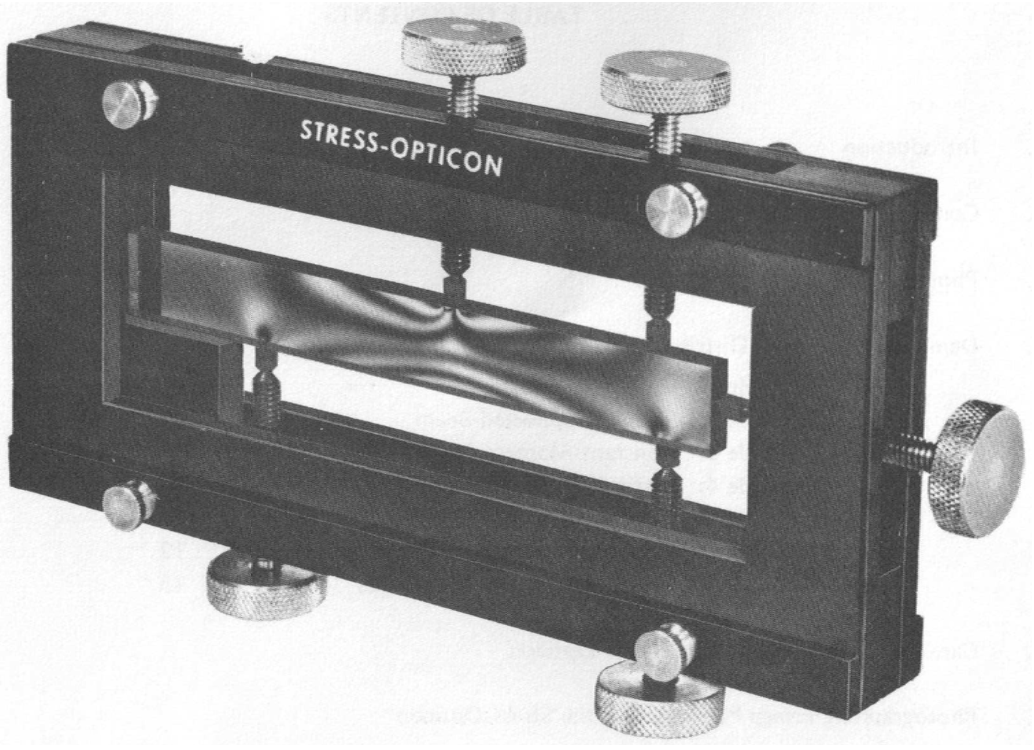
\includegraphics[width=4in]{images/Apparatus}
\caption{The light-field circular polariscope. Image from the Lecture 2 Notes. Copyright 2023 by Thomas Chiou.}
\label{fig:apparatus}
\end{figure}

Using MATLAB, we will analyze the stress equations for a sample with a hole. Our MATLAB scripts will reveal the maxima and minima for the three different types of internal stresses: $\sigma_r$, $\sigma_\theta$, and $\sigma_{r\theta}$. Additionally, we will plot the different stress distributions and the difference between the principal stresses. We will compare the theoretical plot of the principal stress difference with the pictures gathered from the experiment.

\section{Objectives} \label{objectives}
To observe how internal stress changes due to stress discontinuities, also known as stress concentrators, and to analyze theoretical internal stresses due to stress concentrators using MATLAB. An example of a stress concentrator is shown in Figure \ref{fig:stress_concentrators}.

\begin{figure}[htbp]
\centering
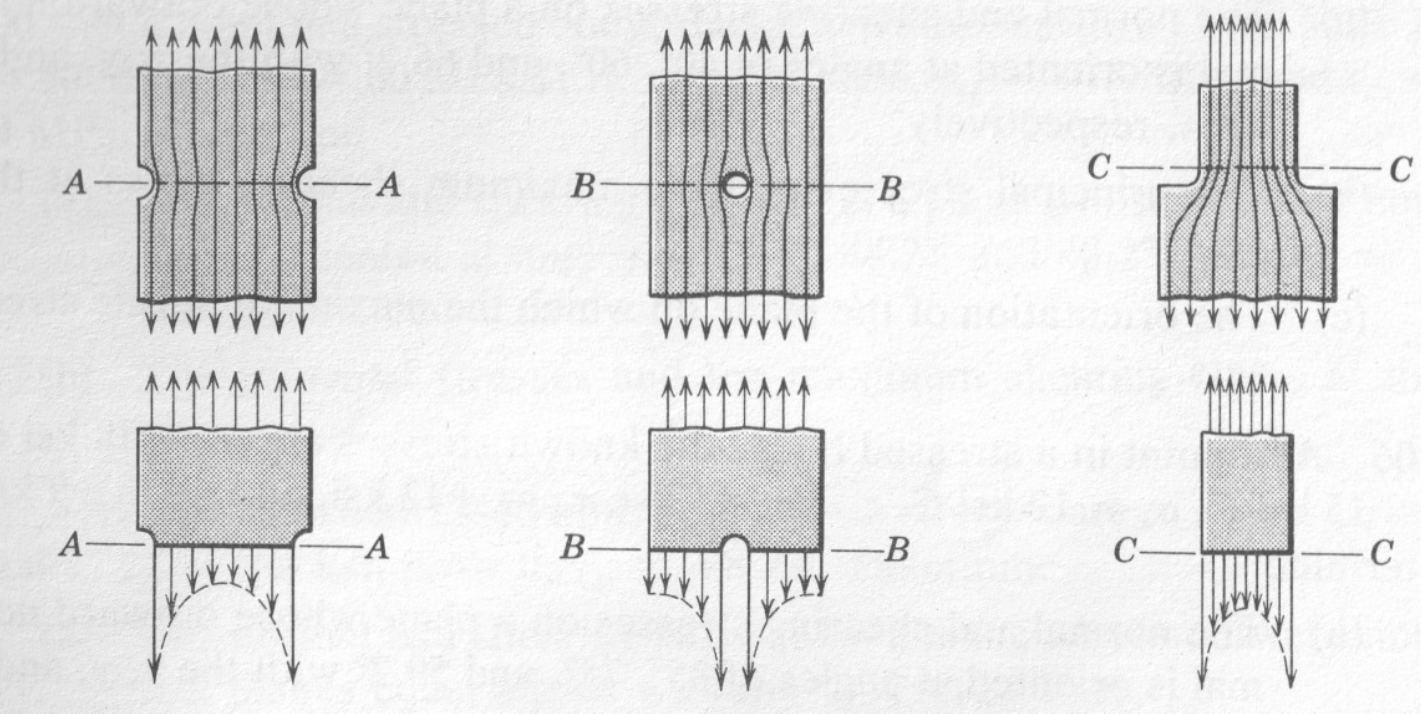
\includegraphics[width=6in]{images/Stress_Concentrators}
\caption{An example of stress discontinuities or concentrators. Image from A. Higdon et al., \textit{Mechanics of Materials}, 4th ed, 1985.}
\label{fig:stress_concentrators}
\end{figure}

\section{Hypothesis} \label{hypothesis}
Due to the photoelastic nature of the material and the polarized sheets, we can photograph the internal stress patterns around the stress concentrators. The difference between the principal stresses will be higher closer to the edges of the discontinuities.

\section{Work Assignments} \label{work_assignments}
Refer to Table \ref{table:work_assignments} for the distribution of work during this lab.

\begin{table}[!htbp]
\caption{Work assignments for AER E 322 Lab 2.}
\begin{center}
	\begin{tabular}{| c | c | c | c |}
		\hline
		\multicolumn{1}{| c |}{\textbf{Task}} & \textbf{Matthew} & \textbf{Peter} & \textbf{Natsuki} \\
		\hline
		\multicolumn{4}{| c |}{\textit{Lab Work}} \\
		\hline
		Date Recording & X & X & X \\
		\hline
		Exp. Setup & X & X & X \\
		\hline
		Exp. Work & X & X & X \\
		\hline
		Exp. Clean-Up & X & X & X \\
		\hline
		\multicolumn{4}{| c |}{\textit{Post Lab}} \\
		\hline
		Question 1 & X & & \\
		\hline
		Question 2 & X & X & \\
		\hline
		Question 3 & X & X & X \\ 
		\hline
		\multicolumn{4}{| c |}{\textit{Report}} \\
		\hline
		Introduction & & X & \\
		\hline
		Objectives & & X & \\
		\hline
		Hypothesis & & X & \\
		\hline
		Materials & & X & \\
		\hline
		Apparatus & & & X \\
		\hline
		Procedures & & & X \\
		\hline
		Data & X & X & X \\
		\hline
		Analysis & X & X & X \\
		\hline
		Conclusion & X & X & \\
		\hline
		Revisions & X & X & \\
		\hline
		Editing & X & & \\
		\hline
	\end{tabular}
\end{center}
\label{table:work_assignments}
\end{table}

\section{Materials} \label{materials}
The materials required for this lab are as follows:

\begin{itemize}
	\item Light-field circular polariscope
	\item Sample with hole
	\item Sample with notch
	\item Sample with arch
\end{itemize}

\section{Apparatus} \label{apparatus}
Figure \ref{fig:notch_2} shows the apparatus with the notched sample loaded with moderate forces.

\begin{figure}[htbp]
\centering
\includegraphics[width=4in,angle=180]{images/notch_2}
\caption{The light-field circular polariscope set up with a semi-loaded notched sample.}
\label{fig:notch_2}
\end{figure}

\section{Procedures} \label{procedures}
We will observe three samples in this lab. To insert a sample into the polariscope, remove the top polarizer and hold the sample in place as you tighten the knobs around the sample. Be careful with the polarizers and samples because they scratch easily. The sample will be ``floating'' between the two polarizers, held by compression with the knobs. The knobs should be evenly spaced around each sample.

Slide the top polarizer back into place, and if there are any fringe patterns visible, loosen the knobs until they disappear. Once the sample is completely clear, slowly tighten the end knob until fringes appear. Do not over-tighten the knob; over-tightening can damage the sample. Stop tightening once the fringe patterns change 2--3 times. Photograph each sample for reference. See Section \ref{data} for images of the fully loaded samples.

\section{Data} \label{data}
The fully loaded samples are shown below in Figures \ref{fig:hole_3}, \ref{fig:notch_3}, and \ref{fig:arch_4}.

\begin{figure}[htbp]
\centering
\includegraphics[width=4in]{images/hole_3}
\caption{The light-field circular polariscope setup with a fully loaded ``hole'' sample.}
\label{fig:hole_3}
\end{figure}

\begin{figure}[htbp]
\centering
\includegraphics[width=4in,angle=180]{images/notch_3}
\caption{The light-field circular polariscope setup with a fully loaded ``notch'' sample.}
\label{fig:notch_3}
\end{figure}

\begin{figure}[htbp]
\centering
\includegraphics[width=4in,angle=180]{images/arch_4}
\caption{The light-field circular polariscope setup with a fully loaded ``arch'' sample.}
\label{fig:arch_4}
\end{figure}

\section{Analysis} \label{analysis}
\textbf{Question 1:}

The normalized stress equations for a sample with a hole in it, derived by dividing both sides of the equation by $\sigma_0$, are shown below.
\begin{align}
\frac{\sigma_r}{\sigma_0}&=\frac{1}{2}\left[\left(1-\frac{a^2}{r^2}\right)-\left(1-\frac{4a^2}{r^2}+\frac{3a^4}{r^4}\right)\cos2\theta\right] \\
\frac{\sigma_\theta}{\sigma_0}&=\frac{1}{2}\left[\left(1+\frac{a^2}{r^2}\right)+\left(1+\frac{3a^4}{r^4}\right)\cos2\theta\right] \label{eqn:norm_sigma_theta} \\
\frac{\tau_{r\theta}}{\sigma_0}&=\frac{1}{2}\left(1+\frac{2a^2}{r^2}-\frac{3a^4}{r^4}\right)\sin2\theta
\end{align}

Given $\theta=\qty{0}{\degree}$ and an arbitrary value for $a$, we can graph the normalized stress curves with respect to $r$, as shown in Figures \ref{fig:norm_sigma_r}, \ref{fig:norm_sigma_theta}, and \ref{fig:norm_tau_rtheta}. The domain of the graphs ranges from $r=a$ to $r=5a$.

\begin{figure}[htbp]
    \centering
    \begin{minipage}{0.45\textwidth}
        \centering
		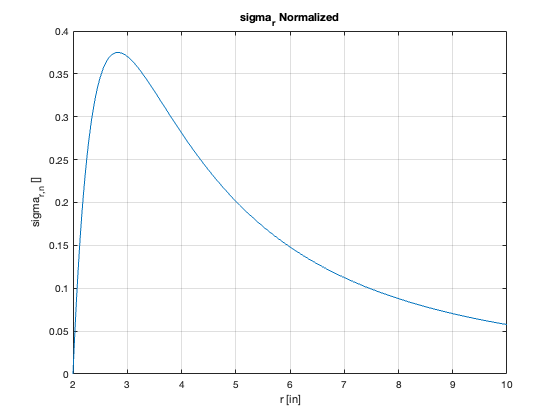
\includegraphics[width=1.0\textwidth]{images/Graphs/sigma_r_normalized}
		\caption{The normalized $\sigma_r$ curve with respect to $r$ from $r=a$ to $r=5a$.}
		\label{fig:norm_sigma_r}
    \end{minipage}\hfill
    \begin{minipage}{0.45\textwidth}
        \centering
		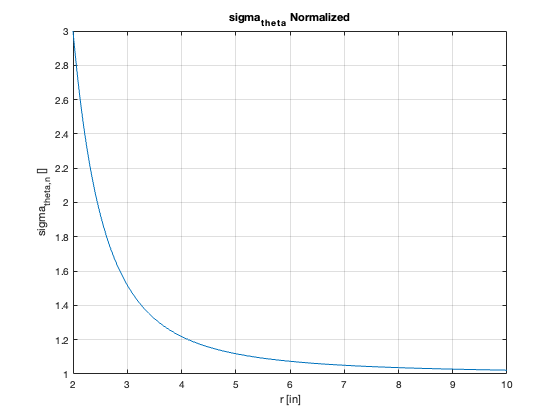
\includegraphics[width=1.0\textwidth]{images/Graphs/sigma_theta_normalized}
		\caption{The normalized $\sigma_\theta$ curve with respect to $r$ from $r=a$ to $r=5a$.}
		\label{fig:norm_sigma_theta}
    \end{minipage}
\end{figure}

\begin{figure}[htbp]
\centering
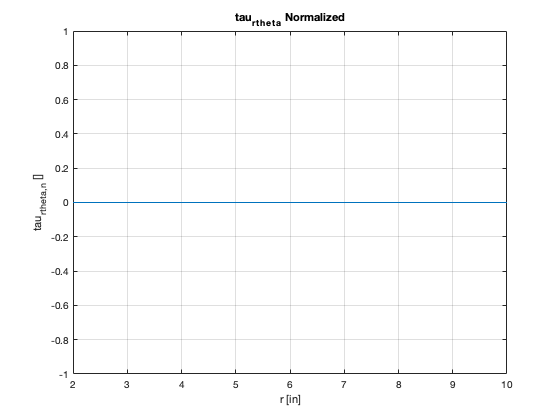
\includegraphics[width=3in]{images/Graphs/tau_rtheta_normalized}
\caption{The normalized $\tau_{r\theta}$ curve with respect to $r$ from $r=a$ to $r=5a$.}
\label{fig:norm_tau_rtheta}
\end{figure}

According to Figures \ref{fig:norm_sigma_r}, \ref{fig:norm_sigma_theta}, and \ref{fig:norm_tau_rtheta}, the internal stress reaches its maximum value in Figure \ref{fig:norm_sigma_theta}, \ie the $\sigma_\theta$ stress contributes most to the internal stress along the line $\theta=\qty{0}{\degree}$. The output from this MATLAB script is as follows:

\begin{tcolorbox}
\begin{verbatim}
Given a = 2 [in]...
sigma_r_n_max = 0.375 [] @ r = 2.83 [in]
sigma_theta_n_max = 3 [] @ r = 2 [in]
tau_rtheta_n = 0 [] @ r = 2 [in]
\end{verbatim}
\end{tcolorbox}

From this output, we observe that the maximum value of the normalized $\sigma_\theta$ curve is \num{3}. Furthermore, the stress concentration factor is defined as

\begin{align}
K\coloneqq\frac{\sigma_\text{max}\text{ or }\tau_\text{max}}{\sigma_0} \label{eqn:def_K}
\end{align}

Plugging in the maximum value of the normalized $\sigma_\theta$ curve into Equation \ref{eqn:norm_sigma_theta}, we get the equations

\begin{align}
\frac{\sigma_\text{max}}{\sigma_0}&=3 \\
\sigma_\text{max}&=3\sigma_0 \label{eqn:sigma_max}
\end{align}

We can now substitute Equation \ref{eqn:sigma_max} into Equation \ref{eqn:def_K}, and we see that the stress concentration factor, $K$, is

\begin{align}
K&=\frac{3\sigma_0}{\sigma_0} \\
K&=3
\end{align}

Figures \ref{fig:norm_sigma_r} and \ref{fig:norm_sigma_theta}, show that the stress rapidly decreases as the measured point of stress moves further from the boundary of the hole. This matches hypothetical observations that the stress magnified at the boundary of discontinuities within a material. In other words, this significantly magnified stress near the surface of a material discontinuity is why nominal imperfections can grow to be catastrophic.

\textbf{Question 2:}

Consider the internal stresses at the boundary of a hole within a sample, \ie $r=a$. It can be shown that $\sigma_r=0$, $\sigma_\theta=\sigma_0\left(1+2\cos2\theta\right)$, and $\tau_{r\theta}=0$. Given these conditions, we can find a ``singular point'' where all internal stresses in the material vanish. For this to be true, $\sigma_\theta$ must be equal to \num{0}, as shown below.

\begin{align}
0&=\sigma_0\left(1+2\cos2\theta\right) \\
-\frac{1}{2}&=\cos2\theta \\
\frac{1}{4}&=\cos^2\theta \\
\theta&=\cos^{-1}\left({\pm\frac{1}{2}}\right) \\
\theta&=\frac{\pi}{3}+2{\pi}n,\frac{5\pi}{3}+2{\pi}n,\frac{2\pi}{3}+2{\pi}n,\frac{4\pi}{3}+2{\pi}n\text{, for any integer }n \label{eqn:theta}
\end{align}

As shown in Equation \ref{eqn:theta}, at the boundary of the hole, the angles \qty{60}{\degree}, \qty{120}{\degree}, \qty{240}{\degree}, and \qty{300}{\degree} have no internal stress.

\textbf{Question 3:}

By substituting arbitrary values for $\sigma_0$ and $a$, \eg $\sigma_0=1$ and $a=2$, we can graph the stress distributions of $\sigma_r$, $\sigma_\theta$, and $\tau_{r\theta}$. These graphs, generated in MATLAB, are shown in Figures \ref{fig:sigma_r}, \ref{fig:sigma_theta}, and \ref{fig:tau_rtheta}.

\begin{figure}[htbp]
    \centering
    \begin{minipage}{0.45\textwidth}
        \centering
		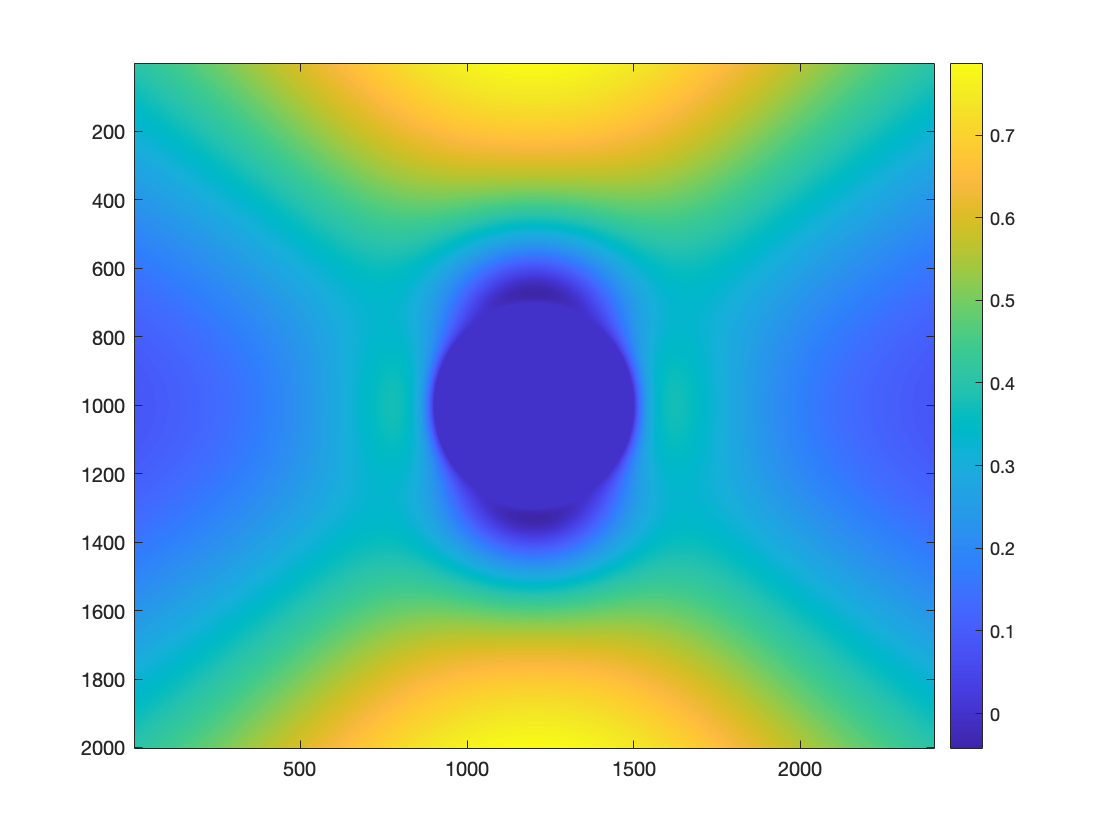
\includegraphics[width=1.0\textwidth]{images/Graphs/sigma_r}
		\caption{The stress distribution of $\sigma_r$ plotted with the MATLAB command \texttt{imagesc}.}
		\label{fig:sigma_r}
    \end{minipage}\hfill
    \begin{minipage}{0.45\textwidth}
        \centering
		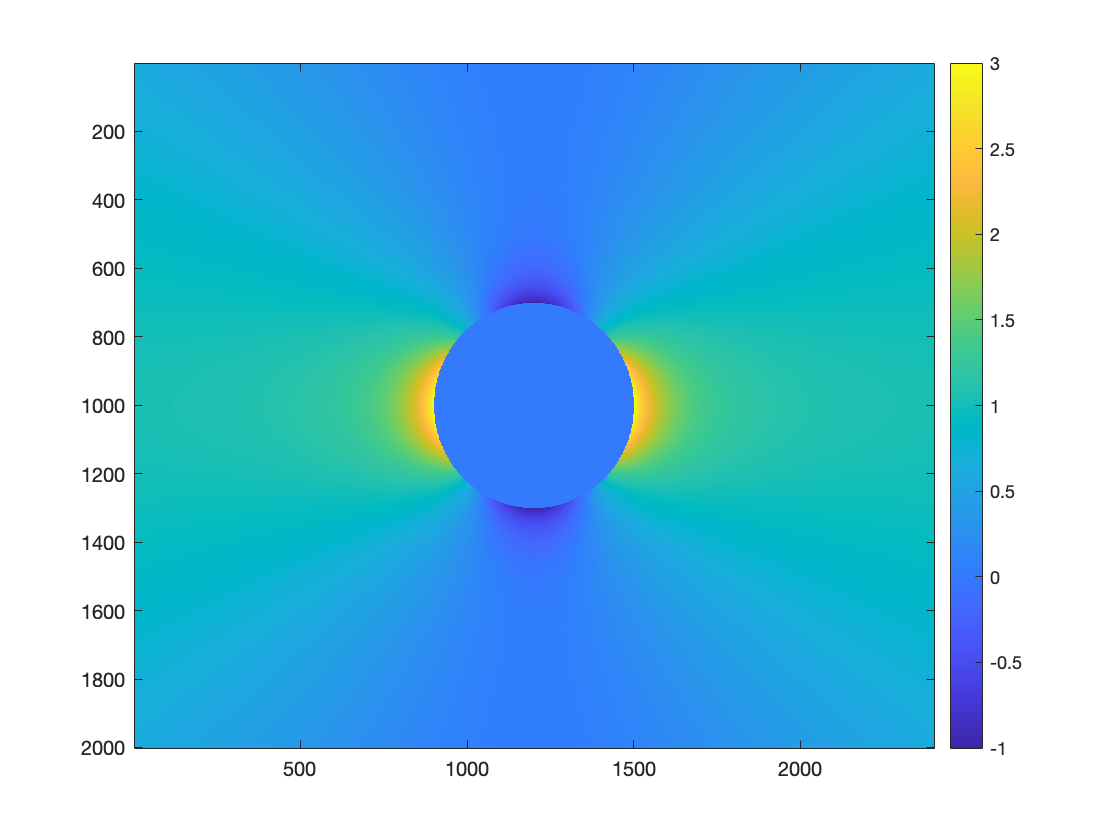
\includegraphics[width=1.0\textwidth]{images/Graphs/sigma_theta}
		\caption{The stress distribution of $\sigma_\theta$ plotted with the MATLAB command \texttt{imagesc}.}
		\label{fig:sigma_theta}
    \end{minipage}
\end{figure}

\begin{figure}[htbp]
\centering
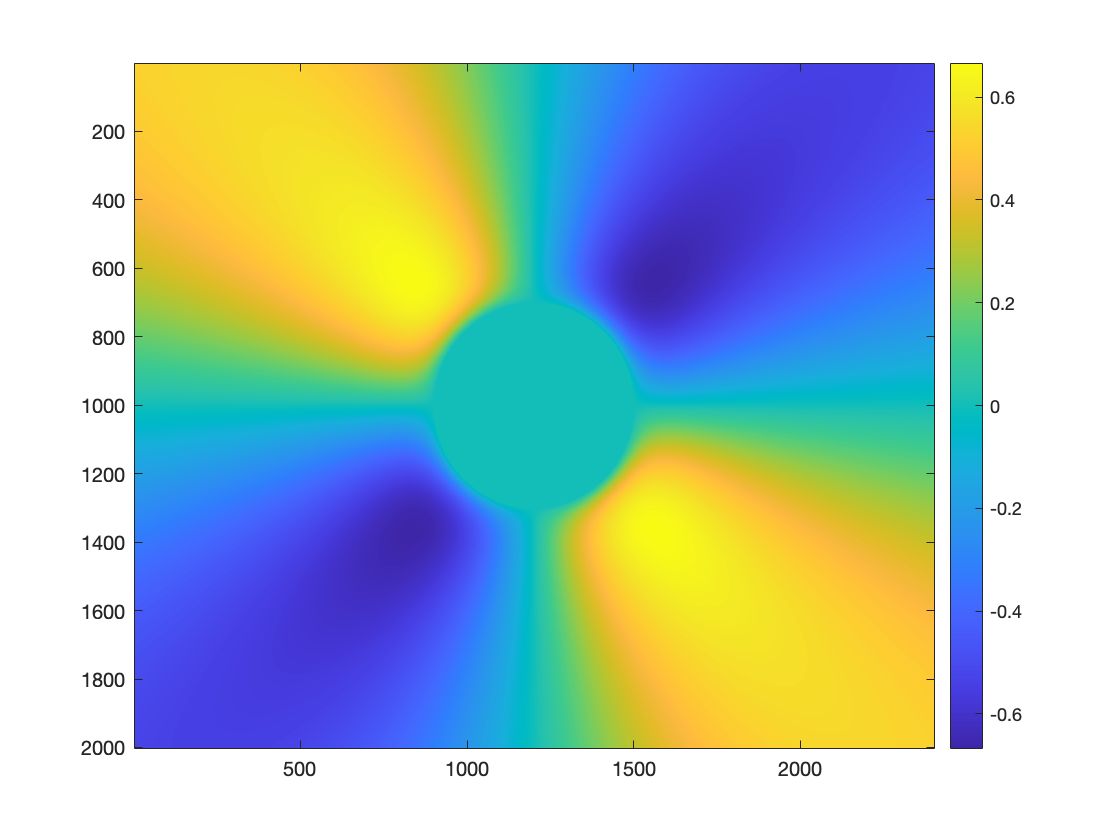
\includegraphics[width=3in]{images/Graphs/tau_rtheta}
\caption{The stress distribution of $\tau_{r\theta}$ plotted with the MATLAB command \texttt{imagesc}.}
\label{fig:tau_rtheta}
\end{figure}

Using the values of $\sigma_r$, $\sigma_\theta$, and $\tau_{r\theta}$ from these MATLAB graphs, we can calculate the difference in the principal stresses, $\sigma_{p1}-\sigma_{p2}$, with the equation

\begin{align}
\sigma_{p1}-\sigma_{p2}=2\sqrt{\left(\frac{\sigma_r-\sigma_\theta}{2}\right)^2+\tau_{r\theta}^2}
\end{align}

The graph of the difference in principal stresses is shown in Figure \ref{fig:principal_stress_diff}.

\begin{figure}[htbp]
\centering
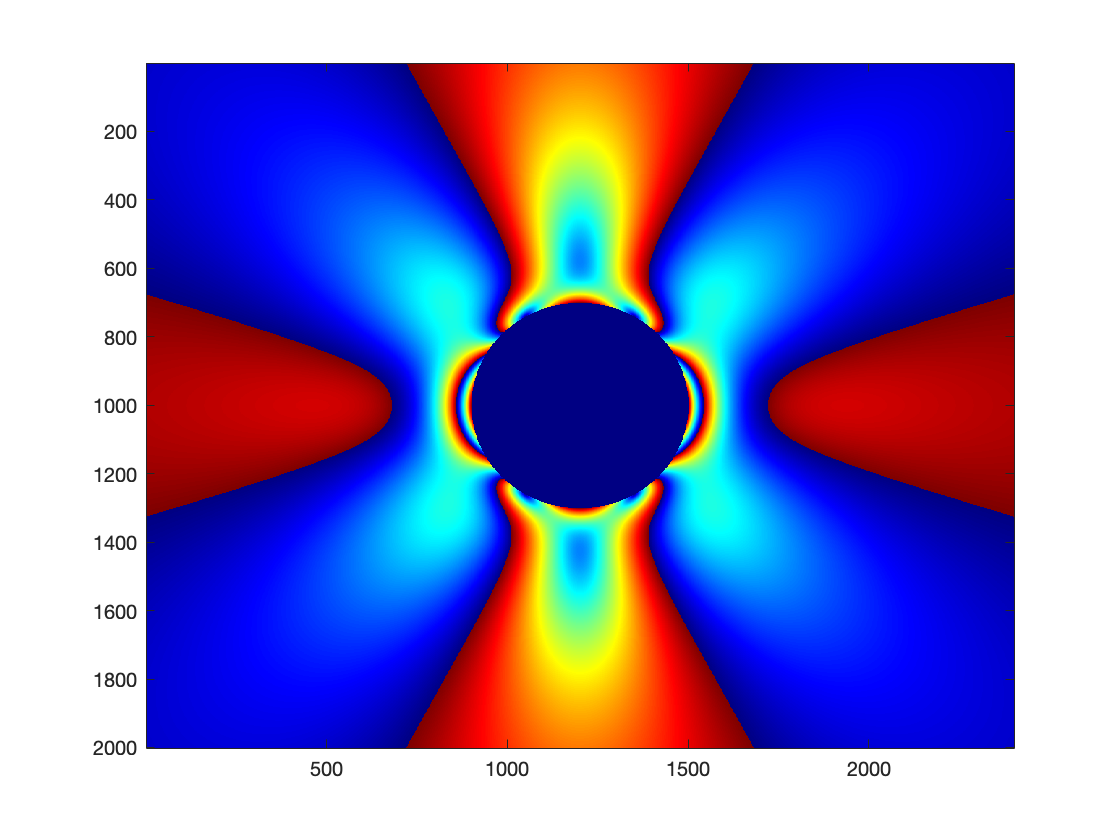
\includegraphics[width=4in]{images/Graphs/principal_stress_diff}
\caption{The stress distribution of $\sigma_{p1}-\sigma_{p2}$ plotted with the MATLAB command \texttt{imagesc}.}
\label{fig:principal_stress_diff}
\end{figure}

By comparing Figure \ref{fig:principal_stress_diff} to our experimental photo of the sample with a hole in it, Figure \ref{fig:hole_3}, we can see similarities between the theoretical stress distribution and the actual photoelastic stress distribution, specifically, if you rotate Figure \ref{fig:hole_3} \qty{90}{\degree}. Perhaps the most notable resemblance comes from the stress rings at $\theta=\qty{0}{\degree},
\qty{180}{\degree}$ in Figure \ref{fig:principal_stress_diff} compared to the stress rings visible on the top and bottom of the hole (closest to the long edges) in Figure \ref{fig:hole_3}. You can also see in Figure \ref{fig:hole_3} the development of the stresses shown at $\theta=\qty{90}{\degree},\qty{240}{\degree}$ of the hole in Figure \ref{fig:principal_stress_diff}.

\section{Conclusion} \label{conclusion}
In this lab, we used a light-field circular polariscope with three different types of samples to visually demonstrate the effect of stress concentrators on internal stress. Using MATLAB, we analyzed the normalized internal stress curves and used the \texttt{imagesc} function to plot colored stress distributions that matched the stress rings we observed in our experimental photographs.

\end{document}
